% !TeX root = origami-activities-en.tex

\section{Teachers' guide}

\subsection{Background}

Origami is the ancient art of paper folding. Origami began to develop when paper was invented in $105$ CE. In $1930$ modern origami was developed by Akira Yoshizawa ($1911$--$2005$). Yoshizawa developed a method of graphically recording the process of folding. In addition, Yoshizawa developed novel methods of folding and solved geometric problems using origami. In the $1950$'s origami became widely known in the United States, where researchers investigated connections between origami and other fields, such as mathematics, medicine and technology.

\subsection{The axioms of origami}

Research into the mathematics of origami began in the $1980$'s. There are seven axioms called the \emph{Huzita-Hatori Axioms} that describe the possible geometric operations during the process of paper folding. The first six axioms were found by the mathematician Humiaki Huzita in $1989$. The set of axioms was completed with a seventh axiom found by the mathematician Koshiro Hatori in $2001$. 

The axioms are expressed in terms of point and lines. The lines are straight lines created by folding a sheet of paper. In the diagrams, folds are indicated by dashed lines.

\textbf{Axiom $1$} Given two points $P_1,P_2$, there is a single fold that passes through them.
% Axiom 1
\begin{center}
\vspace{-1ex}
\begin{tikzpicture}[scale=.9]
\coordinate (P1) at (3,6);
\coordinate (P2) at (4,3);
\fill (P1) circle (1.5pt) node[below left] {$P_1$};
\fill (P2) circle (1.5pt) node[below left] {$P_2$};
\draw[thick,dashed] ($(P1)!-.2!(P2)$) -- ($(P1)!1.5!(P2)$);
\draw[very thick,dotted,->,bend left=35] (5,5) to (2,4);
\end{tikzpicture}
\end{center}

\textbf{Axiom $2$} Given two points $P_1,P_2$, there is a single fold that places $P_1$ onto $P_2$.

% Axiom 2
\begin{center}
\vspace{-1ex}
\begin{tikzpicture}[scale=.9]
\coordinate (P1) at (3,5);
\coordinate (P2) at (5,1);
\fill (P1) circle (1.5pt) node[above left] {$P_1$};
\fill (P2) circle (1.5pt) node[below right] {$P_2$};
\draw[thick,dashed] (2,2) -- (7,5);
\draw[very thick,dotted,->,bend left=35] (3.2,4.8) to (5,1.2);
\end{tikzpicture}
\end{center}

\textbf{Axiom $3$} Given two lines $l_1,l_2$, there is a fold that places $l_1$ onto $l_2$.

% Axiom 3
\begin{center}
\begin{tikzpicture}[scale=1]
\draw (1,2) -- node[near start,above,xshift=-4pt] {$l_1$} (3,6);
\draw (2,1) -- node[near start,below] {$l_2$} (8,4);
\draw[thick,dashed] (1,1) -- (6,6);
\draw[very thick,dotted,->,bend left=35] (2.2,4.2) to (3.9,2.1);
\end{tikzpicture}
\end{center}

There are two cases: (a) if the lines are parallel, the line created by the fold will be parallel to the two lines and equidistant from them; (b) if the lines intersect, the line created by the fold is one of the two bisectors of the vertical angles.

%\vspace{14ex}

\textbf{Axiom $4$} Given a point $P$ and a line $l$, there is a single fold perpendicular to $l$ that passes through $P$.

\begin{center}
\begin{tikzpicture}[scale=1]
\coordinate (L1a) at (3,2);
\coordinate (L1b) at (5,6);
\draw[thick] (L1a) -- node[very near start,right,yshift=-4pt] {$l$} ($(L1a)!1.15!(L1b)$);
\fill (3,5.5) circle (2pt) node[above right] {$P$};
\draw[thick,dashed] (2,6) -- (8,3);
\coordinate (intersection) at (4.4,4.8);
\draw[rotate=-30] (intersection) rectangle +(8pt,8pt);
\draw[very thick,dotted,->,bend left=50] (5.4,6.3) to (3.7,3);
\end{tikzpicture}
\end{center}

%\vspace{14ex}

\textbf{Axiom $5$} Given two points $P_1,P_2$ and a line $l$, there is a fold that places $P_1$ onto $l$ and passes through $P_2$. (There may be zero, one or two such folds as explained in Activity~4.)

% Axiom 5
\begin{center}
\begin{tikzpicture}[scale=.9]
\coordinate (P1) at (1,4);
\coordinate (P2) at (4,3);
\fill (P1) circle (1.5pt) node[above left] {$P_1$};
\fill (P2) circle (1.5pt) node[below right] {$P_2$};
\draw[thick,dashed] (2.5,-1.5) -- (4.6,4.8); %($(3,0)!-.15!(5,6)$) -- (5,6);
\draw[thick] (1,-1) -- node[above] {$l$} ($(1,-1)!1.15!(7,2)$);
\coordinate (P3) at (7,2);
\fill (P3) circle (1.5pt) node[below right] {$P_1'$};
\draw[->,very thick,dotted,bend left=40] ($(P1)+(.2,.15)$) to ($(P3)+(-.2,.15)$);
\end{tikzpicture}
\end{center}

\newpage

\textbf{Axiom $6$} Given two points $P_1,P_2$ and two lines $l_1,l_2$, there is a fold that simultaneously places $P_1$ onto $l_1$ and $P_2$ onto $l_2$. (There may be zero, one, two or three such folds as explained in Activity~5.)

% Axiom 6
\begin{center}
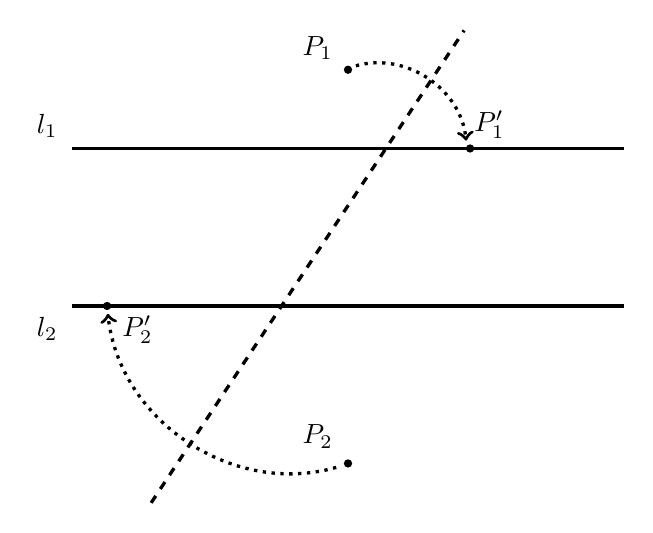
\begin{tikzpicture}[scale=.5]
\coordinate (P1) at (0,4);
\fill (P1) circle (3pt) node[above left,xshift=-2pt] {$P_1$};
\coordinate (P2) at (0,-6);
\fill (P2) circle (3pt) node[above left,xshift=-2pt,yshift=2pt] {$P_2$};
\coordinate (P1P) at (3.1,2);
\fill (P1P) circle (3pt) node[above right,xshift=-2pt] {$P_1'$};
\coordinate (P2P) at (-6.12,-2);
\fill (P2P) circle (3pt) node[below right,xshift=2pt] {$P_2'$};
\draw[very thick] (-7,2) -- node[very near start,above,xshift=-34pt] {$l_1$} (7,2);
\draw[very thick] (-7,-2) -- node[very near start,below,xshift=-34pt] {$l_2$} (7,-2);
\draw[very thick,dashed] (-5,-7) -- (2.95,5);
\draw[very thick,dotted,->,bend left=50] (.2,4.1) to (3,2.2);
\draw[very thick,dotted,->,bend left=50] (-.3,-6.1) to (-6.1,-2.2);
\end{tikzpicture}
\end{center}

\textbf{Axiom $7$} Given a point $P$ and two lines $l_1,l_2$, there is a fold that places $P$ onto $l_1$ and is perpendicular to $l_2$.

% Axiom 7
\begin{center}
\begin{tikzpicture}[scale=.6]
\coordinate (P1) at (5,3);
\fill (P1) circle (2pt) node[below left] {$P$};
\coordinate (P1P) at (2.75,5.25);
\fill (P1P) circle (2pt) node[left,xshift=-4pt] {$P'$};
\draw[very thick] (1,0) -- node[very near start,right,xshift=2pt] {$l_1$} (3,6);
\draw[very thick,name path=l2] (8,3) -- node[very near start,right,xshift=-2pt,yshift=6pt] {$l_2$} (5,6);
\draw[thick] ($(1,0)!-.15!(3,6)$) -- ($(1,0)!1.34!(3,6)$);
\draw[thick] ($(8,3)!-.3!(5,6)$) -- ($(8,3)!1.65!(5,6)$);
\draw[very thick,dashed,name path=fold] (-.5,-.25) -- (7.5,7.75);
\path [name intersections = {of = fold and l2, by = {perp}}];
\draw[rotate=-45] (perp) rectangle +(8pt,8pt);
\draw[very thick,dotted,->,bend right=50] (5.1,3.2) to (3,5.2);
\end{tikzpicture}
\end{center}

%%%%%%%%%%%%%%%%%%%%%%%%%%%%%%%%%%%%%%%%%%%%%%%%%%%%%%%%%%%%%%%%%%
%%%%%%%%%%%%%%%%%%%%%%%%%%%%%%%%%%%%%%%%%%%%%%%%%%%%%%%%%%%%%%%%%%
%%%%%%%%%%%%%%%%%%%%%%%%%%%%%%%%%%%%%%%%%%%%%%%%%%%%%%%%%%%%%%%%%%

\subsection{The mathematics of origami}

The first axiom systems was \emph{Euclidean geometry}, named after the third-century mathematician who collected and extended geometrical theorems and proofs in the book \emph{The Elements}. Euclidean geometry was based on construction by straightedge (an unmarked ruler) and compass. The straightedge can construct a line that goes through two existing points; the compass can construct a circle from a given point (its center) and a given line segment (its radius).

There were three problems for which the Greeks were unable to find constructions with straightedge and compass: (1) trisecting an arbitrary angle into three equal parts; (2) squaring a circle: given a circle, construct a square with the same area; (3) doubling a cube: given a cube, construct another cube with twice the volume. In addition, they were unable to construct a regular heptagon (a regular polygon with seven sides).

It was not until the $19$-th century that the reason for their failures was understood. A straightedge and compass can only construct values that are obtainable from a line segment defined to have length $1$ and the operations of $\{+,-,\times, \div,\surd\}$. Squaring a circle is certainly impossible because it requires constructing the value $\pi$ which cannot be obtained from any algebraic formula. The other problems require the construction of cube roots which is impossible. For example, doubling a cube requires the construction of the value $\sqrt[3]{2}$.

The basic constructions of Euclidean geometry are: bisecting a line segment, bisecting an angle, copying a line segment, copying an angle, constructing a perpendicular to a line from a point not on the line, constructing a perpendicular to a line from a point on the line. All these constructions can be performed in origami using Axioms~$1$--$5$. The power of origami comes from Axiom~$6$: placing two points on two lines turns out to enable constructions that cannot be performed using straightedge and compass, in particular, constructions that require the computation of cube roots.

\subsection{Proof by folding}

Throughout the activities, the students will be asked to ``prove by folding.'' The intention is that the student perform a fold that will explain why a claim is true. Before each activity, the teacher must explain to the students when a fold proves a claim. We here present an example of a simple explanation that should be shown to the students before the activities (or as necessary).

% Axiom 2
\begin{wrapfigure}{r}{.4\textwidth}
\begin{center}
\vspace{-4ex}
\begin{tikzpicture}[scale=1.1]
\coordinate (P1) at (2,2);
\coordinate (P2) at (6,4);
\coordinate (mid1) at ($(P1)!.5!(P2)$);
\coordinate (mid2) at ($(P1)!.5!(P2)+(-1,2)$);
\fill (mid2) circle(1pt) node[above right] {$A$};
\draw (P1) -- node[fill=white] {$a$} (mid2) -- node[fill=white] {$a$} (P2);
\draw[very thick,dashed] ($(mid1)!-.9!(mid2)$) --
  node[very near end,left,xshift=-6pt,yshift=8pt] {$l$}
  ($(mid1)!1.4!(mid2)$);
\fill (P1) circle(1pt) node[above left] {$P_1$};
\fill (P2) circle(1pt) node[above,yshift=2pt] {$P_2$};
\draw[very thick,dotted,->,bend right=50] (2,1.8) to (6,3.8);
\end{tikzpicture}
\end{center}	
\end{wrapfigure}
\textbf{Proof by folding}: Consider Axiom~$2$: given two points $P_1,P_2$, there is a single fold that places $P_1$ onto $P_2$. Look at the line constructed by this fold and an arbitrary point $A$ on the line. The fold does not move the point, so the line segment $\overline{AP_1}$ is placed onto the line segment $\overline{AP_2}$, so their lengths are equal. We have proved by folding that if the endpoints of a line segment are copied onto the endpoints of another segment then their lengths are equal.


